  Here we consider a standard epidemic model to describe the dynamics of a 
disease. We use optimal control techniques to find a vaccination
schedule for the disease. Goal is to minimize the number of infectious 
persons and the overall cost of the vaccine during a fixed time period. 

  Here $S(t)$,$I(t)$,$R(t)$ respectively denote the number of susceptible 
infectious, and recovered (immune) individuals at time $t$. The model also 
consider a class that represent the number of exposed $E(t)$. 
Then the whole population $N$ is given by $N(t) = S(t) + E(t) + I(t) + R (t)$,
and obeys the last equation of model \eqref{eqn:epidemics_lenhart}.

The control $u(t)$ is a fraction of susceptible individual being 
vaccinated per unit of time. Since vaccination of the entire susceptible 
population is impractical, the model considers $0 \leq u(t) \leq 0.9$. 

Hence, the optimal control problem reads\em parameters in 
\Cref{tbl:epidemics_lenhart}.


\begin{equation} \label{eqn:epidemics_lenhart}
  \begin{aligned}
    \min_{u} & \int_{0}^{T} AI(t) + u^{2}(t) dt,
    \\
    \text{subject to}
    \\
      \dot{S}(t) &=
          bN(t) - dS(t) - cS(t)I(t) - u(t)S(t), \quad S(0) = S_0 \geq 0,   \\
      \dot{E}(t) &=
          cS(t)I(t) - (e + d)E(t), \quad E(0) = E_0 \geq 0,    \\
      \dot{I}(t) &=
          eE(t) - (g + a +d)I(t), \quad I(0) = I_0 \geq 0,     \\
      \dot{R}(t) &=
          gI(t) -dR(t) + u(t)S(t), \quad R(0) = R_0 \geq 0,    \\
      \dot{N}(t) &=
          (b - d)N(t) - aI(t), \quad N(0) = N_0 \geq 0,        \\
  \end{aligned}
\end{equation}

\begin{table}[htb]
  \begin{center}
    \begin{tabular}{rll}
      \toprule
        & \multicolumn{1}{c}{\textbf{Description}} 
        & \textbf{Simulation values}
        \\
      \midrule
        $b$
          & Recruitment rate
          & \num{0.525}
        \\
        $a$, $d$ 
          & Disease and natural death rates
          & \num{0.2}, \num{0.5}
        \\
        $c$
          & Incidence of disease
          & \num{0.0001}
        \\
        $e$
          & Rate at which the exposed 
          & \num{0.5}
          \\
          & individuals become infectious
        \\
        $g$
          & Recovering rate
          & \num{0.1}
        \\
        $A$
          & Vaccination cost
          & \num{0.1}
        \\
        $T$
          & Final time
          & \num{20.0}
        \\
        \\
        && 
        \multicolumn{1}{c}{
          \textbf{Initial conditions}
        }
        \\
        \cmidrule{3-3}
          &&
            $S(0) = \num{1000}$, $E(0) = \num{100}$
          \\
          &&
            $I(0) = \num{50}$, $R(0) = \num{15}$
        \\
      \bottomrule
    \end{tabular}
    \caption{Parameters and simulation values of the epidemic model
      \eqref{eqn:epidemics_lenhart}}
    \label{tbl:epidemics_lenhart}
  \end{center}
\end{table}

 Note that the disease free state is 
$(bN/d,0,0,0)$.

The Hamiltonian for this problem is
\begin{align*}
    H(t,x,u,\lambda) &= AI + u^{2} + \left< \lambda , g \right> \\
                     &= AI + u^{2} + \sum_{i \in J} \lambda_{i}g_{i}
\end{align*}
where $J = \{S, E, I, R\}$ and $g_i$ is the right hand side of the corresponding
equation.

%---------%---------%---------%---------%---------%---------%---------%---------
\begin{theorem} 
    There exists an optimal control $u^{*}$ and corresponding solutions, \break
    $S^{*}, E^{*}, I^{*}, T^{*}, N^{*}$ that maximizes $J(u)$ over $[0, 1]$. 
    Also, there exists adjoint functions, $\lambda_{i}, i \in J$, such that
    \begin{align*}
         \dot{\lambda}_{S} &=
            \lambda_{S}\left(d + cI + u \right) - \lambda_{E}cI - 
            \lambda_{R}u   \\
        \dot{\lambda}_{E} &=
            \lambda_{E}(e + d) - \lambda_{I}e  \\
        \dot{\lambda}_{I} &=
            (\lambda_{S} - \lambda_{E})cS + \lambda_{I}(g + a +d) - \lambda_{R}g
            \lambda_{N}a\\
        \dot{\lambda}_{R} &=    \lambda_{R}d  \\
        \dot{\lambda}_{N} &=
            - \lambda b - \lambda_{R}d  (b - d)
    \end{align*}
\end{theorem}

\begin{figure}[tbh!]
\centering
	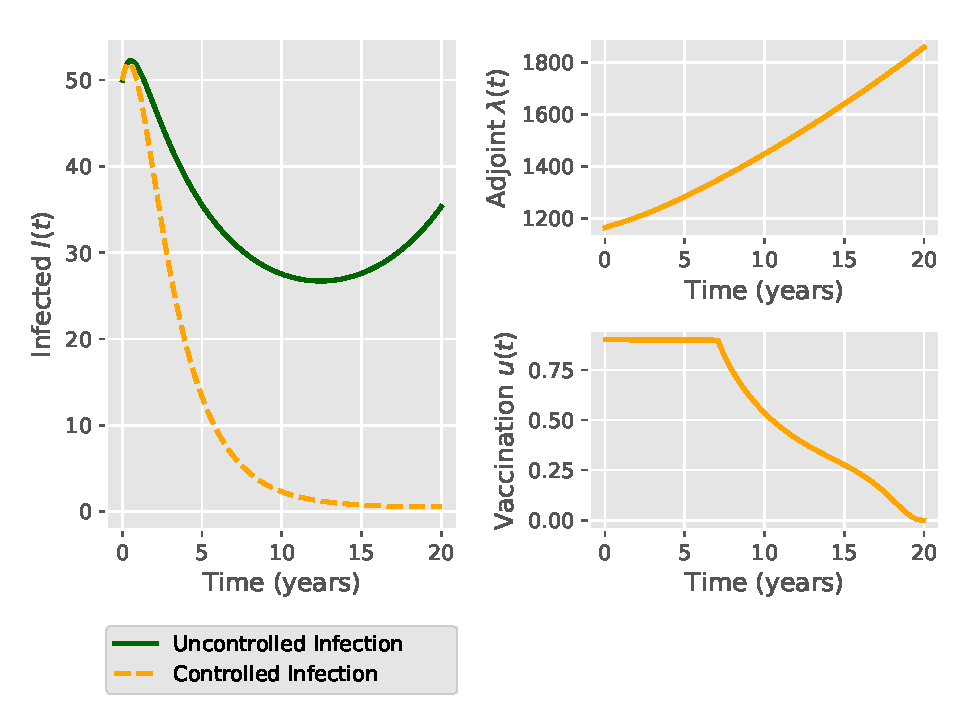
\includegraphics{./Figures/epidemics_lenhart_lab7}
	\caption{Likening between the controlled and uncontrolled Infected 
	 population.  At right, we show the optimal infected state agains the 
	 dynamics without 
	 control. At right we present the corresponding adjoint function $\lambda$ 
	 and the optimal control.}
\label{fig:epidemicslenhartlab7}
\end{figure}
